\documentclass{beamer}

\usepackage[utf8]{inputenc}
\usepackage{default}

\mode<presentation>
%{ \usetheme{boxes} }


\usetheme{Madrid}

\usepackage{times}
\usepackage{graphicx}
\usepackage{tabulary}
\usepackage{listings}
\usepackage{verbatimbox}
\usepackage{graphicx}
\usepackage{lmodern}
\usepackage[absolute,overlay]{textpos}
\usepackage{pgfpages}
\usepackage{color}
\usepackage{multicol}
\usepackage{multimedia}
\usepackage{hyperref}
\usepackage{amsmath}
\pgfdeclareimage[height=1.0cm]{logo_rcc}{icons/ANL_RGB-01.jpg}
\setlength{\TPHorizModule}{1mm}
\setlength{\TPVertModule}{1mm}
\newcommand{\RCCLogo}{
\begin{textblock}{14}(1.5,1.5)
  \pgfuseimage{logo_rcc}
\end{textblock}
}


\definecolor{mycolorcli}{RGB}{53,154,26}
\definecolor{mycolorcode}{RGB}{0,0,255}
\definecolor{mycolordef}{RGB}{255,0,0}
\definecolor{mycolorlink}{RGB}{184,4,255}


\title{\huge{Compression pipeline}}
\author{Igor Yakushin}
\date{October 23, 2019}

%\definecolor{ChicagoMaroon}{RGB}{0,49,101}
\definecolor{ChicagoMaroon}{RGB}{4,78,156}

\setbeamercolor{title}{bg=ChicagoMaroon}

\begin{document}

\setbeamertemplate{navigation symbols}{}

\setbeamercolor{fcolor}{fg=white,bg=ChicagoMaroon}
\setbeamertemplate{footline}{
\begin{beamercolorbox}[ht=4ex,leftskip=1.4cm,rightskip=.3cm]{fcolor}
\hrule
\vspace{0.1cm}
   \hfill \insertshortdate \hfill \insertframenumber/\inserttotalframenumber
\end{beamercolorbox}
}

\setbeamercolor{frametitle}{bg=ChicagoMaroon,fg=white}

\begin{frame}
\RCCLogo
\titlepage
\end{frame}

\section{Pipeline}

\begin{frame}[fragile]
  \frametitle{Pipeline}
\begin{center}
 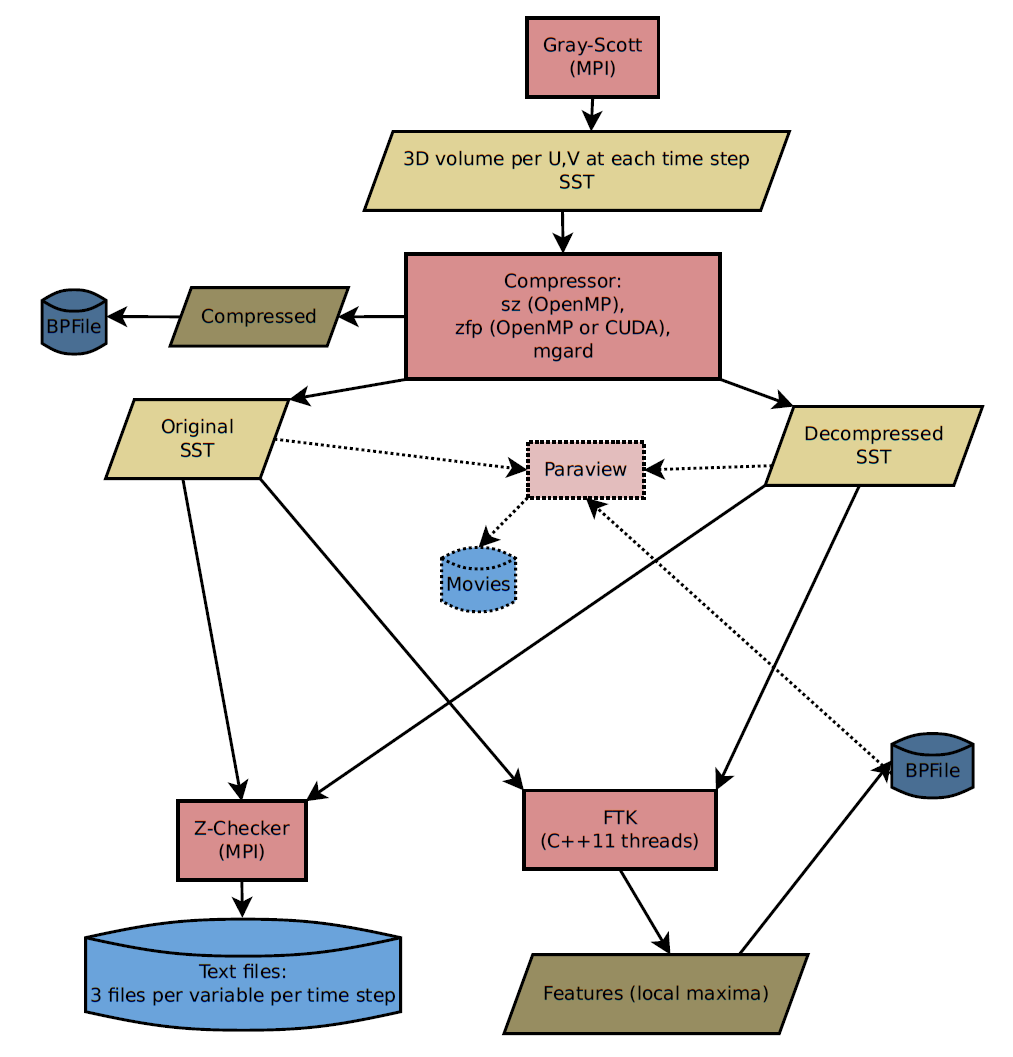
\includegraphics[width=7.6cm]{graphs/pipeline.png}
\end{center}
\end{frame}


\begin{frame}[fragile]
  \frametitle{Pipeline}
  \begin{itemize}
  \item Gray-Scott simulation
    \begin{itemize}
    \item currently uses $256^3$ grid
    \item two variables, $U$ and $V$, evolve according to two coupled non-linear PDEs, generating non-trivial patterns
    \item initial condition: $U$ is 1 everywhere except for the cube in the middle where it is 0.25; $V$ is 0 everywhere except for the
      same cube in the middle where it is 0.33
    \item some random noise is added to $U$ at each iteration, its amplitude is a parameter
    \item 1000 time steps
    \item every 100 steps a checkpoint is created and sent via ADIOS2 SST stream to compressor
    \end{itemize}
  \end{itemize}
\end{frame}

\begin{frame}[fragile]
  \frametitle{Pipeline}
  \begin{itemize}
  \item Compressor
    \begin{itemize}
    \item uses one of the following algorithms: SZ, ZFP, MGARD
    \item compresses and decompresses the data
    \item compressed data is written to a file with enough metadata to decompress
    \item original and lossy (compressed/decompressed) data are sent via ADIOS2 SST streams to ZChecker and FTK to evaluate the quality of the compression
    \end{itemize}
  \item ZChecker
    \begin{itemize}
    \item gets original and lossy data
    \item runs its usual comparison and stores the results in usual ZChecker format: 3 text files per iteration, per variable
    \end{itemize}
  \end{itemize}
\end{frame}

    
\begin{frame}[fragile]
  \frametitle{Pipeline}
  \begin{itemize}
  \item FTK
    \begin{itemize}
    \item gets original and lossy data
    \item finds the number of local maxima on each variable on both datasets
    \item computes the distance as normalized difference between the number of local maxima for each variable
    \item local maxima coordinates and values, number of maxima, distances are stored in ADIOS2 BP4 files.
    \end{itemize}
  \item Cheetah/Savanna is used to set up and run the experiments
  \item ParaView
    \begin{itemize}
    \item used for debugging purposes offline
    \item compared original and lossy data side by side to visualize time evolution and spacial distribution of $U$ and $V$
      and show local maxima found by FTK
    \item see the link to movies on $32^3$ grid in references
    \end{itemize}
  \end{itemize}
\end{frame}

    

\section{FTK}

\begin{frame}[fragile]
  \frametitle{FTK}
  \begin{itemize}
  \item We tried to use FTK as a feature detector to compare the original and lossy data
  \item As a distance, we use normalized difference of the number of local maxima
  \item Next slide shows how this distance depends on the tolerance that is a parameter
    for each compressor
  \item ZFP and MGARD have only one input parameter to control the compression
  \item SZ can use several kinds of tolerance parameters, here by ``tolerance'' we mean the default one: \verb|pw_relBoundRatio|
  \end{itemize}
\end{frame}

\subsection{Distance}
\begin{frame}[fragile]
  \frametitle{FTK: distance}
  
  There is no clear correlation between tolerance and FTK distance
  
  \begin{center}
    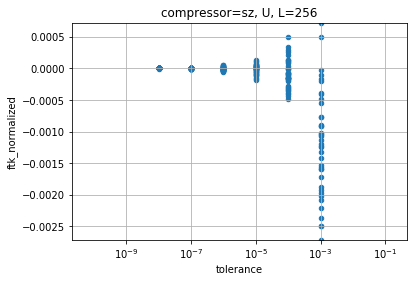
\includegraphics[width=3.7cm]{graphs/ndistance_sz_U.png}
    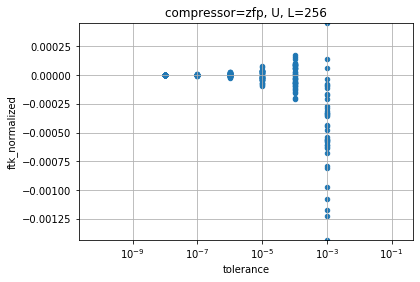
\includegraphics[width=3.7cm]{graphs/ndistance_zfp_U.png}
    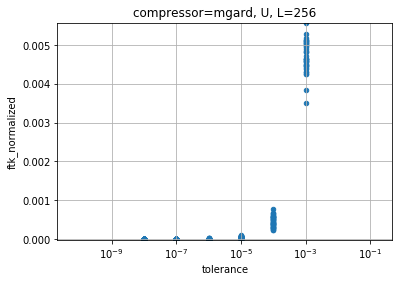
\includegraphics[width=3.7cm]{graphs/ndistance_mgard_U.png}
    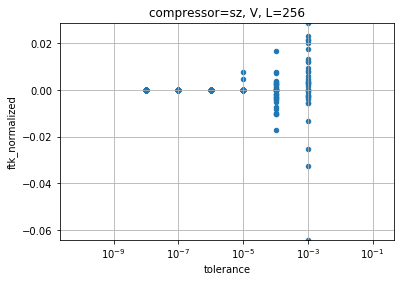
\includegraphics[width=3.7cm]{graphs/ndistance_sz_V.png}
    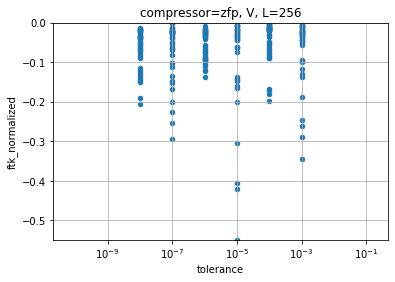
\includegraphics[width=3.7cm]{graphs/ndistance_zfp_V.png}
    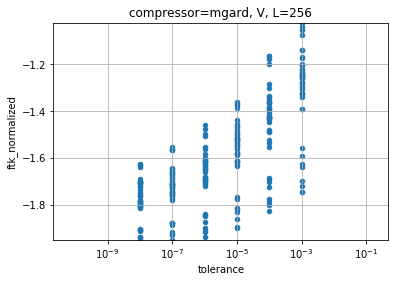
\includegraphics[width=3.7cm]{graphs/ndistance_mgard_V.png}    
  \end{center}
\end{frame}

\subsection{ZChecker}
\begin{frame}[fragile]
  \frametitle{FTK: ZChecker measurements}

  Varios ZChecker's measurements behave as expected

  \begin{center}
    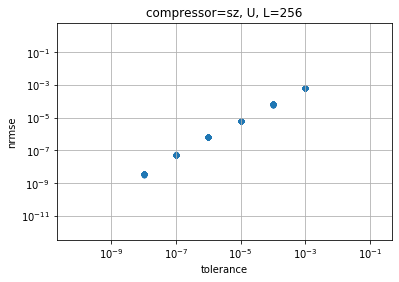
\includegraphics[width=3.7cm]{graphs/rmse_sz_U.png}
    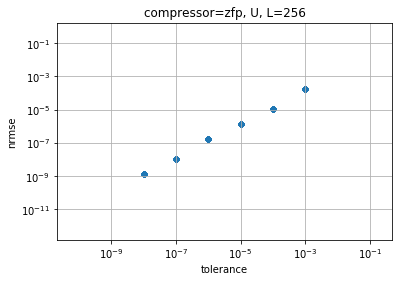
\includegraphics[width=3.7cm]{graphs/rmse_zfp_U.png}
    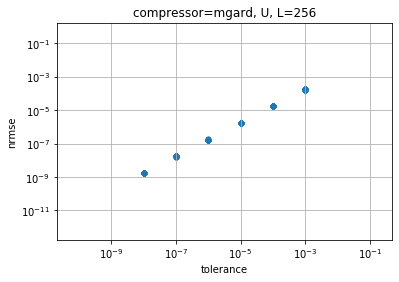
\includegraphics[width=3.7cm]{graphs/rmse_mgard_U.png}
    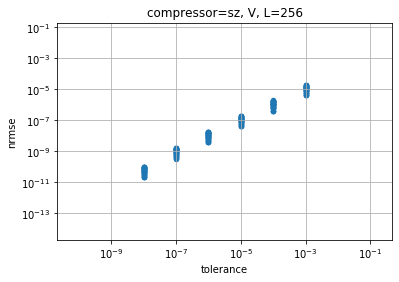
\includegraphics[width=3.7cm]{graphs/rmse_sz_V.png}
    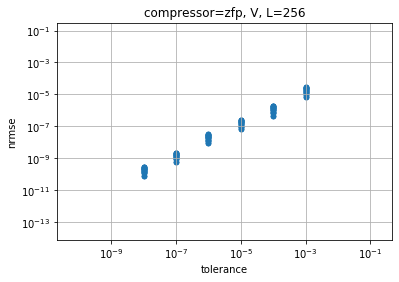
\includegraphics[width=3.7cm]{graphs/rmse_zfp_V.png}
    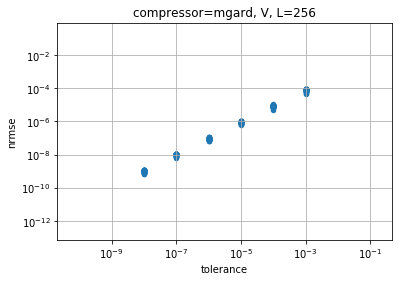
\includegraphics[width=3.7cm]{graphs/rmse_mgard_V.png}        
  \end{center}

\end{frame}

\subsection{Number of maxima for $noise = 10^{-2}$}
\subsubsection{SZ}
\begin{frame}[fragile]
  \frametitle{FTK: number of maxima for $noise = 10^{-2}$, SZ }

{\tiny
\begin{table}[H]
\centering
\begin{tabular}{|r|r|r|r|r|}
\hline
tolerance &         number of max, original &         number of max, lossy &       difference & normalized difference \\
\hline
  1.0e-08 &           828279 &        828279 &             0.0 &       0.00e+00 \\
\hline
  1.0e-07 &           825165 &        825166 &            -1.0 &      -1.21e-06 \\
\hline
  1.0e-06 &           825966 &        825996 &           -30.0 &      -3.63e-05 \\
\hline
  1.0e-05 &           824939 &        825007 &           -68.0 &      -8.24e-05 \\
\hline
  1.0e-04 &           827345 &        827418 &           -73.0 &      -8.82e-05 \\
\hline
  1.0e-03 &           824677 &        825416 &          -739.0 &      -8.96e-04 \\
\hline
\end{tabular}
\caption{SZ, U, $step = 1000$, $noise = 10^{-2}$}
\label{sz_u_table}
\end{table}
}

{\tiny
Notice: the number of maxima in the original data above is only 20 times smaller than the total number of points in the volume.
}

{\tiny
\begin{table}[H]
\centering
\begin{tabular}{|r|r|r|r|r|}
\hline
tolerance &         number of max, original &         number of max, lossy &       difference & normalized difference \\
\hline

  1.0e-08 &              981 &           981 &             0.0 &       0.00e+00 \\
\hline
  1.0e-07 &             1004 &          1004 &             0.0 &       0.00e+00 \\
\hline
  1.0e-06 &              917 &           917 &             0.0 &       0.00e+00 \\
\hline
  1.0e-05 &             1003 &          1003 &             0.0 &       0.00e+00 \\
\hline
  1.0e-04 &              987 &           985 &             2.0 &       2.03e-03 \\
\hline
  1.0e-03 &              941 &           942 &            -1.0 &      -1.06e-03 \\
\hline
\end{tabular}
\caption{SZ, V, $step = 1000$, $noise = 10^{-2}$}
\label{sz_v_table}
\end{table}
}

  
\end{frame}


\begin{frame}[fragile]
  \frametitle{FTK: number of maxima for $noise = 10^{-2}$, SZ }

  \begin{itemize}
  \item For $V$ the number of maxima is of reasonable size and almost identical between the original
    and lossy data; a small difference appears only at high tolerance $10^{-4}$
  \item The difference between the graphs and the tables is coming from two sources:
    \begin{itemize}
    \item In the tables only the last checkpoint is shown while on the graph all 10 checkpoints
    \item In the tables the results shown only for 64 MPI ranks for Gray-Scott and ZChecker (this experiment was done on theta)
      while on the graphs 4 combinations of $(32, 64)$ ranks are tried
    \end{itemize}
  \end{itemize}
\end{frame}

\subsubsection{ZFP}
\begin{frame}[fragile]
  \frametitle{FTK: number of maxima for $noise = 10^{-2}$, ZFP }

  {\tiny
    \begin{table}[H]
      \centering
      \begin{tabular}{|r|r|r|r|r|}
        \hline
        tolerance &         number of max, original &         number of max, lossy &       difference & normalized difference \\
        \hline
        1.0e-08 &           825854 &        825854 &             0.0 &       0.00e+00 \\
        \hline
        1.0e-07 &           827774 &        827777 &            -3.0 &      -3.62e-06 \\
        \hline
        1.0e-06 &           826774 &        826766 &             8.0 &       9.68e-06 \\
        \hline
        1.0e-05 &           826603 &        826629 &           -26.0 &      -3.15e-05 \\
        \hline
        1.0e-04 &           825891 &        825910 &           -19.0 &      -2.30e-05 \\
        \hline
        1.0e-03 &           826406 &        826549 &          -143.0 &      -1.73e-04 \\
        \hline
      \end{tabular}
      \caption{ZFP, U, $step = 1000$, $noise = 10^{-2}$}
      \label{zfp_u_table}
    \end{table} 
  }

  {\tiny
    \begin{table}[H]
      \centering
      \begin{tabular}{|r|r|r|r|r|}
        \hline
        tolerance &         number of max, original &         number of max, lossy &       difference & normalized difference \\
        \hline
        
        1.0e-08 &              914 &           933 &           -19.0 &      -2.06e-02 \\
        \hline
        1.0e-07 &             1064 &          1092 &           -28.0 &      -2.60e-02 \\
        \hline
        1.0e-06 &             1018 &          1117 &           -99.0 &      -9.29e-02 \\
        \hline
        1.0e-05 &              987 &           994 &            -7.0 &      -7.08e-03 \\
        \hline
        1.0e-04 &              964 &           978 &           -14.0 &      -1.44e-02 \\
        \hline
        1.0e-03 &              975 &           997 &           -22.0 &      -2.23e-02 \\
        \hline
      \end{tabular}
      \caption{ZFP, V, $step = 1000$, $noise = 10^{-2}$}
      \label{zfp_v_table}
    \end{table}
  }

  {\tiny
    While the results for $U$ are similar to those of SZ, the results for $V$ show no clear correlation between the number of maxima and the tolerance, and this is correctly reflected in more or less constant absolute value of distance
  }
\end{frame}



\subsubsection{MGARD}
\begin{frame}[fragile]
  \frametitle{FTK: number of maxima for $noise = 10^{-2}$, MGARD }

  {\tiny
\begin{table}[H]
\centering
\begin{tabular}{|r|r|r|r|r|}
\hline
tolerance &         number of max, original &         number of max, lossy &       difference & normalized difference \\
\hline

  1.0e-08 &           826506 &        826502 &             4.0 &       4.84e-06 \\
\hline
  1.0e-07 &           825201 &        825204 &            -3.0 &      -3.64e-06 \\
\hline
  1.0e-06 &           826299 &        826302 &            -3.0 &      -3.63e-06 \\
\hline
  1.0e-05 &           827031 &        827031 &             0.0 &       0.00e+00 \\
\hline
  1.0e-04 &           824480 &        824156 &           324.0 &       3.93e-04 \\
\hline
  1.0e-03 &           825847 &        821624 &          4223.0 &       5.13e-03 \\
\hline
\end{tabular}
\caption{MGARD, U, $step = 1000$, $noise = 10^{-2}$}
\label{mgard_u_table}
\end{table}

  }

  {\tiny
\begin{table}[H]
\centering
\begin{tabular}{|r|r|r|r|r|}
\hline
tolerance &         number of max, original &         number of max, lossy &       difference & normalized difference \\
\hline
  1.0e-08 &              979 &          9540 &         -8561.0 &      -1.63e+00 \\
\hline
  1.0e-07 &              955 &          7887 &         -6932.0 &      -1.57e+00 \\
\hline
  1.0e-06 &              927 &          6472 &         -5545.0 &      -1.50e+00 \\
\hline
  1.0e-05 &              900 &          4816 &         -3916.0 &      -1.37e+00 \\
\hline
  1.0e-04 &              934 &          3720 &         -2786.0 &      -1.20e+00 \\
\hline
  1.0e-03 &              966 &          3058 &         -2092.0 &      -1.04e+00 \\
\hline
\end{tabular}
\caption{MGARD, V, $step = 1000$, $noise = 10^{-2}$}
\label{mgard_v_table}
\end{table}
  }
 {\tiny
  Notice: for $V$ MGARD lossy data has 10 times more local maxima than the original data and as the tolerance increases,
  the distance decreases which is opposite to what we saw for other compression algorithms. Apparently MGARD introduces its own
  artifacts and the higher the required compression precision, the more artifacts are introduced.
 }
 
\end{frame}


\subsection{Number of maxima for $noise = 0$}
\begin{frame}[fragile]
  \frametitle{FTK: number of maxima for $noise = 0$ }
  \begin{itemize}
  \item Reducing the noise amplitude from $10^{-2}$ to $10^{-5}$ does not significantly change the results:
    still the number of local maxima in the original data for $U$ is only about 20 times less than the number of points in
    the volume - anything, no matter how small, that is larger than its immediate neighbors is considered to be local maxima
  \item Therefore, let us try to turn the noise completely off
  \item We shall consider only two values for tolerance for simplicity
  \end{itemize}
\end{frame}


\begin{frame}[fragile]
  \frametitle{FTK: number of maxima for $noise = 0$ }

  {\tiny
\begin{table}[H]
\centering
\begin{tabular}{|r|r|r|r|r|}
\hline
tolerance &  number of max, original &  number of max, lossy &  difference & normalized difference \\
\hline
  1.0e-08 &               50 &           645 &          -595.0 &      -1.72e+00 \\ \hline
  1.0e-03 &               50 &           452 &          -402.0 &      -1.61e+00 \\  \hline
\end{tabular}
\caption{SZ, U, step=500, $noise=0$}
\label{sz_u_n0}
\end{table}

\begin{table}[H]
\centering
\begin{tabular}{|r|r|r|r|r|}
\hline
tolerance &  number of max, original &  number of max, lossy &  difference & normalized difference \\
\hline
  1.0e-08 &              558 &           614 &           -56.0 &      -9.57e-02 \\ \hline
  1.0e-03 &              558 &           551 &             7.0 &       1.27e-02 \\ \hline
\end{tabular}
\caption{SZ, V, step=500, $noise=0$}
\label{sz_v_n0}
\end{table}

 \begin{table}[H]
\centering
\begin{tabular}{|r|r|r|r|r|}
\hline
tolerance &  number of max, original &  number of max, lossy &  difference & normalized difference \\
\hline 
  1.0e-08 &               50 &           219 &          -169.0 &      -1.27e+00 \\ \hline
  1.0e-03 &               50 &           235 &          -185.0 &      -1.31e+00 \\ \hline
\end{tabular}
\caption{ZFP, U, step=500, $noise=0$}
\label{zfp_u_n0}
\end{table}

\begin{table}[H]
\centering
\begin{tabular}{|r|r|r|r|r|}
\hline
tolerance &  number of max, original &  number of max, lossy &  difference & normalized difference \\
\hline 
  1.0e-08 &              558 &           579 &           -21.0 &      -3.70e-02 \\ \hline
  1.0e-03 &              558 &           617 &           -59.0 &      -1.01e-01 \\ \hline
\end{tabular}
\caption{ZFP, V, step=500, $noise=0$}
\label{zfp_v_n0}
\end{table}

 



  }

  
\end{frame}


\begin{frame}[fragile]
  \frametitle{FTK: number of maxima for $noise = 0$ }

  {\tiny

 \begin{table}[H]
\centering
\begin{tabular}{|r|r|r|r|r|}
\hline
tolerance &  number of max, original &  number of max, lossy &  difference & normalized difference \\
\hline 

  1.0e-08 &               50 &          4687 &         -4637.0 &      -1.96e+00 \\ \hline
  1.0e-03 &               50 &          1224 &         -1174.0 &      -1.85e+00 \\ \hline
\end{tabular}
\caption{MGARD, U, step=500, $noise=0$}
\label{mgard_u_n0}
\end{table}

\begin{table}[H]
\centering
\begin{tabular}{|r|r|r|r|r|}
\hline
tolerance &  number of max, original &  number of max, lossy &  difference & normalized difference \\
\hline 

  1.0e-08 &              558 &          6480 &         -5922.0 &      -1.68e+00 \\ \hline
  1.0e-03 &              558 &          1860 &         -1302.0 &      -1.08e+00 \\ \hline
\end{tabular}
\caption{MGARD, V, step=500, $noise=0$}
\label{mgard_v_n0}
\end{table}

  }


  \begin{itemize}
  \item While setting $noise = 0$ got rid of unmanageable number of local maxima in the original data, it did not address
    compression/decompression artifacts generated in the lossy data
  \item Hanqi suggested to try to use Gaussian filtering to precondition data before applying FTK - almost finished implementing it
  \end{itemize}
  
\end{frame}

\section{Timing pipeline components on Summit and Theta}

\subsection{Offloading Gray-Scott to GPU with Kokkos}

\begin{frame}[fragile]
  \frametitle{Offloading Gray-Scott to GPU with Kokkos}
  \begin{itemize}
  \item The original version of Gray-Scott runs on CPU using MPI
  \item To justify using Summit, Gray-Scott was accelerated with Kokkos
  \item The same code - one line change - can be used to offload to GPU on Summit or to use multithreading on Theta
  \end{itemize}

  {\tiny
    \begin{table}[H]
      \centering
      \begin{tabular}{|r||r|r|r|r||r|r|r|}
        \hline
	& CPU & CPU & CPU & CPU & GPU & GPU & GPU\\
        \hline
	MPI ranks & 1 & 8 & 21 & 42 & 1 & 3 & 6\\
        \hline
	compute/rank/iteration, ms & 199,972 & 23,743 & 9,911 & 4968 & 1,819 & 625 & 404\\
        \hline
	write/rank/iteration, ms & 7,597 & 3,414 & 531 & 335 & 7850 & 2887 & 1631\\
        \hline
      \end{tabular}
      \caption{L=512, summit}
      \label{kokkos_512_summit}
    \end{table}
  }
  
  \begin{itemize}
  \item To use Kokkos requires some bleeding edge compiler specifically built to offload to GPU, same applies to OpenMP GPU offloading
  \item I am using LLVM 9.0.0 on Summit
  \item On Theta, while I can build Kokkos version of Gray-Scott, I had some trouble compiling some other components of the pipeline.
    So for now I am using original version of Gray-Scott on Theta.
  \end{itemize}

\end{frame}


\subsection{Gantt chart on Theta}

\begin{frame}[fragile]
  \frametitle{Gantt chart on Theta}

  \begin{center}
    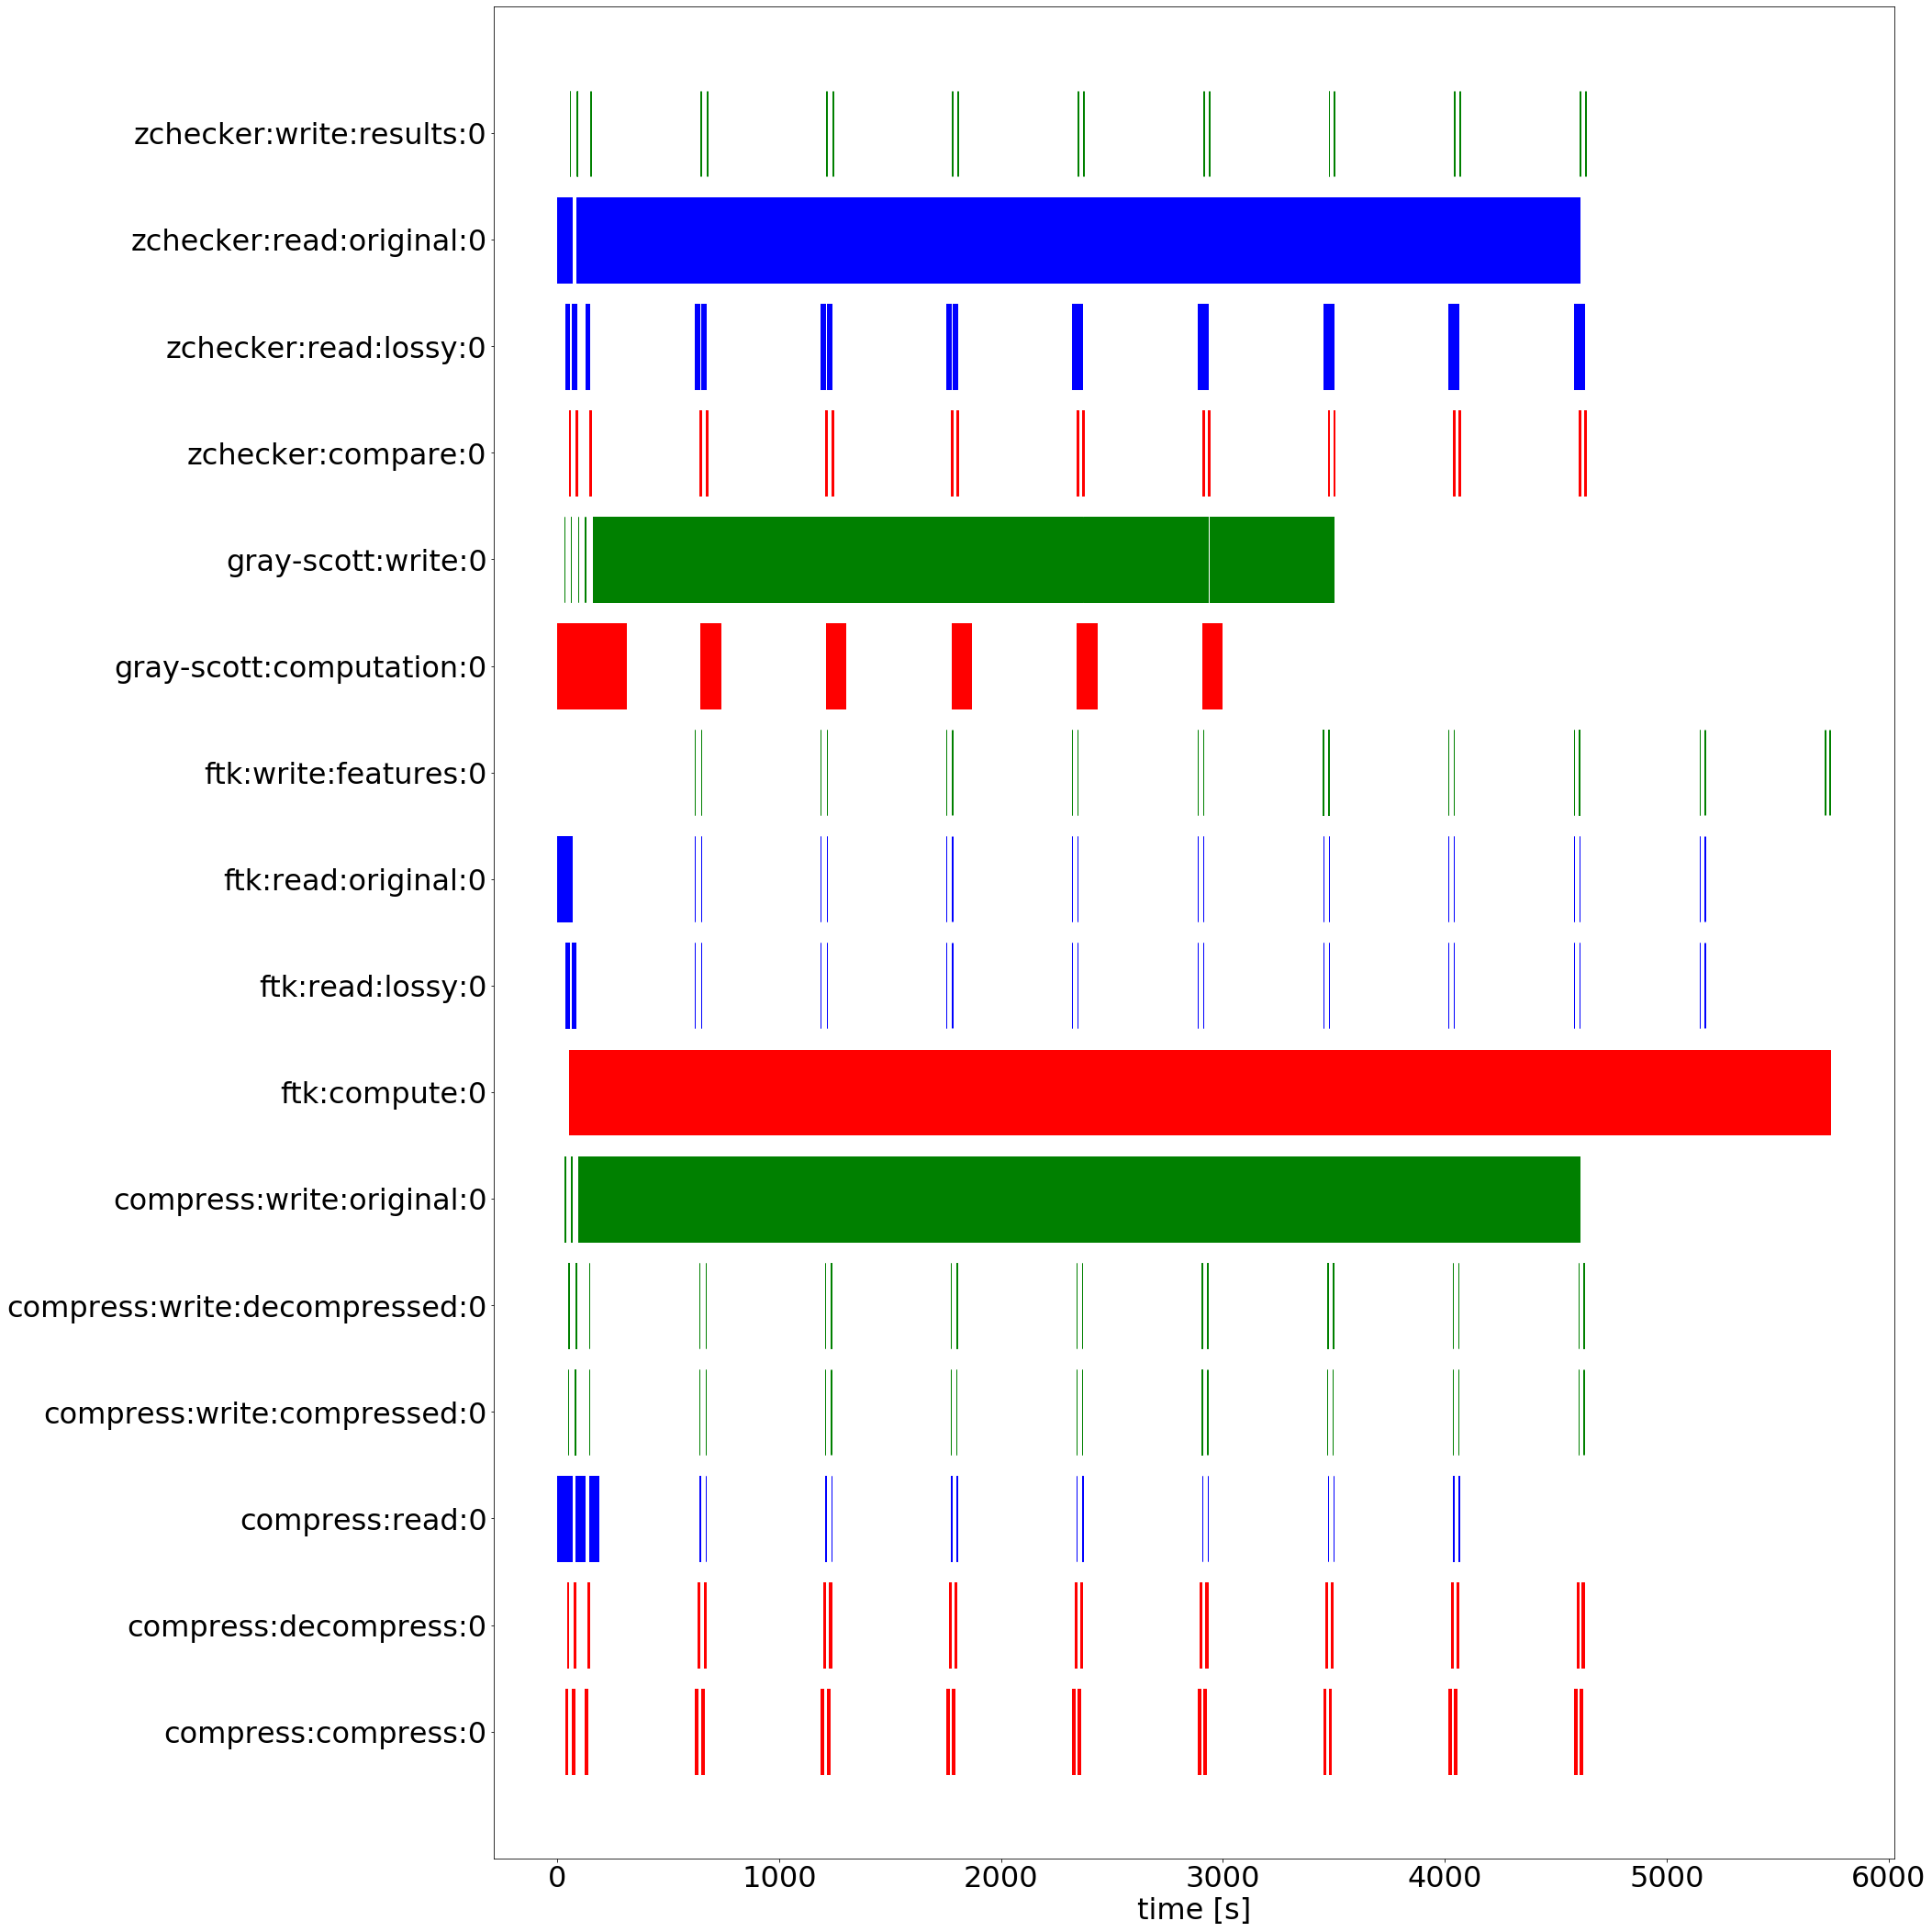
\includegraphics[width=8cm]{graphs/gantt_theta.png}
  \end{center}
\end{frame}


\begin{frame}[fragile]
  \frametitle{Gantt chart on Theta}
  \begin{itemize}
  \item Timing is shown for SZ, $U$, $256^3$ grid
  \item Only one MPI rank of each pipeline component is shown, other ranks have identical timing
  \item Red corresponds to computations: Gray-Scott compute, compression/decompression, ZChecker and FTK comparisons
  \item Green corresponds to write
  \item Blue corresponds to read
  \item Everything is dominated by FTK computations, all other computations take negligible time in comparison
  \item Long times for I/O are misleading. ADIOS2 SST streams are configured in such a way that
    \begin{itemize}
    \item Gray-Scott waits for compressor to pick up its checkpoint before proceeding to the next iteration
    \item compressor waits for ZChecker and FTK to pick up its data before proceeding to the next iteration
    \end{itemize}
  \item As a result, long I/O times are due to waiting for FTK to finish the previous iteration and not due to actually moving bits
  \end{itemize}
\end{frame}


\subsection{adios2.xml}
\begin{frame}[fragile]
  \frametitle{Gantt chart on Theta: adios2.xml}

  \begin{columns}

    \begin{column}{0.5\textwidth}
{\tiny
\begin{verbatim}
<adios-config>
 <io name="SimulationOutput">
  <engine type="SST">
  <parameter key="RendezvousReaderCount" value="1"/>
  <parameter key="QueueLimit" value="1"/>
  <parameter key="QueueFullPolicy" value="Block"/>
 </engine>
</io>
<io name="OriginalOutput">
 <engine type="SST">
  <parameter key="RendezvousReaderCount" value="2"/>
  <parameter key="QueueLimit" value="1"/>
  <parameter key="QueueFullPolicy" value="Block"/>
 </engine>
</io>
<io name="CompressedOutput">
 <engine type="BPFile">
  <parameter key="RendezvousReaderCount" value="1"/>
  <parameter key="QueueLimit" value="1"/>
  <parameter key="QueueFullPolicy" value="Block"/>
 </engine>
</io>
\end{verbatim}
}

    \end{column}

    \begin{column}{0.5\textwidth}

{\tiny
\begin{verbatim}
<io name="DecompressedOutput">
 <engine type="SST">
  <parameter key="RendezvousReaderCount" value="2"/>
  <parameter key="QueueLimit" value="1"/>
  <parameter key="QueueFullPolicy" value="Block"/>
</engine>
</io>
<io name="FTK">
 <engine type="BPFile">
  <parameter key="RendezvousReaderCount" value="1"/>
  <parameter key="QueueLimit" value="1"/>
  <parameter key="QueueFullPolicy" value="Block"/>
 </engine>
</io>
</adios-config>
\end{verbatim}
}
      
    \end{column}
  \end{columns}


\end{frame}




\subsection{Detailed comparison}
\begin{frame}[fragile]
  \frametitle{Detailed comparison}

{\tiny
\begin{table}[H]
\centering
\begin{tabular}{|r|r|r|r|r|r|}
\hline
 & \multicolumn{3}{|c|}{Summit} & \multicolumn{2}{|c|}{Theta} \\
 \hline	
	 & MPI ranks & CPU threads & GPUs & MPI ranks & CPU threads\\
\hline
	Gray-Scott & 2 & 1 & 2 & 64 & 1\\
\hline
	SZ & 1 & 1 & 0 & 1 & 1\\
\hline
	ZFP & 1 & 1 & 0 & 1 & 1\\
\hline
	MGARD & 1 & 1 & 0 & 1 & 1\\
\hline
	ZChecker & 5 & 1 & 0 & 64 & 1\\
\hline
	FTK & 1 & 20 & 0 & 1 & 64\\
\hline
\end{tabular}
\caption{Utilized computational resources}
\label{cresources}
\end{table}
}

{\tiny

\begin{table}[H]
\centering
\begin{tabular}{|r|r|r|}
\hline
	 & Summit & Theta\\
\hline
	Gray-Scott compute & $14 \pm 0.05$ & $32 \pm 0.2$ \\
\hline
	SZ compress & $2.5 \pm 0.05$ & $11 \pm 0.5$ \\
\hline
	SZ decompress  & $2.0 \pm 0.15$ & $ 7.9 \pm 0.5$ \\
\hline
	ZFP compress & $0.4 \pm 0.3 $ & $1.3 \pm 1.1$ \\
\hline
	ZFP decompress & $0.43 \pm 0.35$ & $1.5 \pm 1.2$ \\
\hline
	MGARD compress & $15 \pm 6$ & $72 \pm 48$\\
\hline
	MGARD decompress & $2.2 \pm 0.07$ & $16 \pm 0.7$\\
\hline
	ZChecker compare & $1.9 \pm 0.009$ & $3.5 \pm 0.1$ \\
\hline
	FTK compare & $81 \pm 0.3$ & $560 \pm 0.8$ \\
\hline
\end{tabular}
\caption{Average timing of various pipeline components in seconds.
  Grid size $256^3$. Gray-Scott simulation was run 1000 time steps, saving checkpoints every 100 iterations.
Therefore the averaging was done over 10 samples. The input compression tolerance here is fixed at $10^{-3}$. }
\label{timing}
\end{table}

}

  
\end{frame}


\begin{frame}[fragile]
  \frametitle{Detailed comparison}

  \begin{itemize}
  \item On Summit the whole pipeline fits into a single node
  \item On Theta each component runs on a separate node - 4 nodes

  \item Notice that timing for SZ compression/decompression is measured differently than for ZFP and MGARD:
    SZ times include both $U$ and $V$ variables, while for the other compression algorithms time is measured separately
    for different variables and this is the origin of high std for ZFP and MGARD and higher mean for SZ. This needs to be unified later.

  \item If instead of 64 hardware threads, one uses all 256 hardware threads on theta's KNL node,
    FTK compare time drops from $560$ to $480 \pm 0.6$ seconds.
  \item  If instead of 64 MPI ranks for Gray-Scott on Theta, one uses 32 MPI ranks,
    the run time for 100 iterations increases from $32$ to $62 \pm 0.3$ seconds.

  \item If instead of 64 MPI ranks for ZChecker comparison on theta, one uses 32 MPI ranks,
    the run time increases from $1.9$ to $7 \pm 0.2$ seconds.
  \end{itemize}
\end{frame}


\begin{frame}[fragile]
  \frametitle{Detailed comparison}
  \begin{itemize}
  \item FTK is the biggest bottleneck
  \item MGARD is much slower than other compression algorithms
  \item Theta is much slower than Summit
  \item Possible improvements to timing:
    \begin{itemize}
    \item FTK is called 4 times sequentially for original and lossy data, for $U$ and $V$ - this can be done in parallel using MPI;
      debugging the corresponding version
    \item Currently FTK can only use CPU threads - accelerate it to use GPUs
    \item Hanqi's summer students integrated FTK with MPI - might help on Theta but not on Summit
    \item Recent development in MGARD - it is cudarized now
    \end{itemize}
  \end{itemize}
\end{frame}

\section{TODO}

\begin{frame}[fragile]
  \frametitle{TODO}
  \begin{itemize}
  \item Try to reduce the influence of noise in the original data and compression/decompression artifacts in the lossy data
    on FTK distance by using something like Gaussian filtering
  \item If the above helps, speed up FTK
    \begin{itemize}
    \item Use MPI to call FTK in parallel 4 times
    \item Accelerate FTK on GPU?
    \item Use MPI version of FTK once Hanqi releases it
    \end{itemize}
  \item Try newer accelerated version of MGARD
  \item Benchmark Kokkos and original version of Gray-Scott on Theta
  \item Unify how compression/decompression timing is done for all the compression algorithms
  \item Visualize $256^3$ with ParaView after all the changes since the previous set of movies was generated
  \item Resolve LLVM compiling issues on Theta
  \item Debug OpenMP GPU offloading version of Gray-Scott?
  \item Put the pipeline into Spack? Singularity container?
  \end{itemize}
\end{frame}

%\input{movies.tex}
%\input{next.tex}
\section{References}                                                                                                                                                                 
\begin{frame}[fragile]                                                                                                                                                               
  \frametitle{References}                                                                                                                                                            
{\tiny                                                                                                                                                                               
\begin{verbatim}
Pipeline repo:
https://github.com/CODARcode/cheetah/tree/compression_split/examples/05-gray-scott-compression
Current work page:
https://users.nccs.gov/~iyakushin/compression_pipeline/index.html
Paraview movies:
https://anl.app.box.com/s/c7x29xf49mofmeftwqrlqe4nt6heulyh

K. Mehta, B. Allen, M. Wolf, J. Logan, E. Suchyata, J. Choi, K. Takahashi, I. Yakushin, 
T. Munson, I. Foster, and S. Klasky
A codesign framework for online data analysis and reduction at the exascale. 2019. 
Accepted for presentation at WORKS 2019

The "Parallel Vectors" Operator - A Vector Field Visualization Primitive
Ronald Peikert and Martin Roth

Cheetah/Savanna repo: https://github.com/CODARcode/cheetah

ADIOS2: https://adios2.readthedocs.io

Tao, D., Di, S., Guo, H., Chen, Z., & Cappello, F. (2019). 
Z-checker: A framework for assessing lossy compression of scientific data. 
The International Journal of High Performance Computing Applications, 33(2), 285-303.

Z-checker repo: https://github.com/CODARcode/Z-checker
SZ repo: https://github.com/disheng222/SZ
MGARD repo: https://github.com/CODARcode/MGARD
ZFP repo: https://github.com/LLNL/zfp
FTK repo: https://github.com/CODARcode/ftk

Gray-Scott: https://www.karlsims.com/rd.html
\end{verbatim}
}

\end{frame}

\section{Appendix A: Gray-Scott reaction-diffusion model}

\begin{frame}[fragile]
  \frametitle{Apendix A: Gray-Scott reaction-diffusion model}
  \begin{columns}
    \begin{column}{0.5\textwidth}
      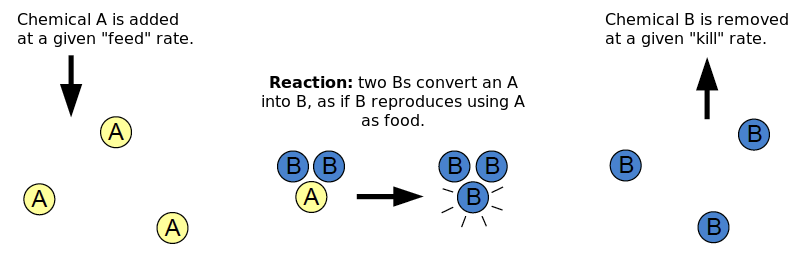
\includegraphics[width=5.5cm]{graphs/reaction.png}
    \end{column}
    \begin{column}{0.5\textwidth}
      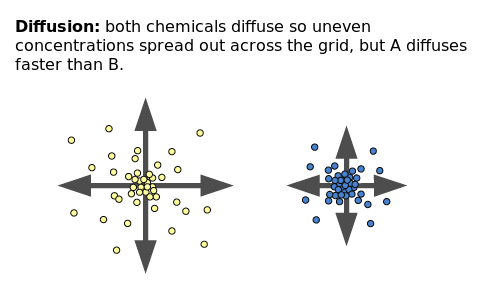
\includegraphics[width=5.5cm]{graphs/diffusion.png}
    \end{column}
  \end{columns}
  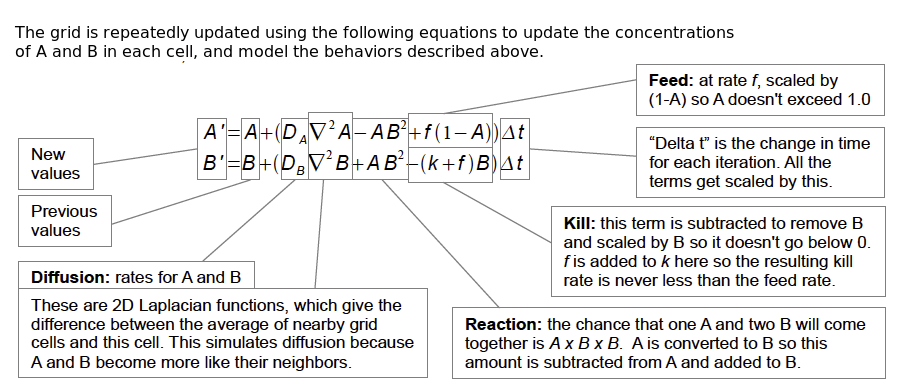
\includegraphics[width=11cm]{graphs/equations.png}  
\end{frame}
\end{document}

